\documentclass[solutions]{esg8012pset} 
  \usepackage{amsmath}
  \usepackage{amssymb}
  \usepackage{enumerate}
  \usepackage{graphicx}
  \usepackage{hyperref}
  %\usepackage{siunitx}
  \providecommand{\uvec}[1]{{\hat{\bf{#1}}}}
  \usepackage{pgf,tikz}
  \usetikzlibrary{arrows}
  \makeatletter
  \newcommand{\interitemtext}[1]{%
    \begin{list}{}
     {\itemindent=0mm\labelsep=0mm
     \labelwidth=0mm\leftmargin=0mm
     \addtolength{\leftmargin}{-\@totalleftmargin}}
      \item #1
    \end{list}
  }
  \makeatother
  \renewcommand{\d}{\,d}
  \providecommand{\norm}[1]{\lVert#1\rVert}
\classname{Physics 8.012} 
\semester{Fall 2010} 
\problemsetnumber{6} 
\date{October 15} 
\duedate{Friday, October 22} 
\readingassignment{Kleppner and Kolenkow, \emph {An Introduction to Mechanics}, Chapter Four} 
\begin{document}
\section*{Problem 1: K\&K 4.2}
\subsection*{Problem}
  A block of mass $m$ slides along a horizontal table with speed $v_0$. At $x = 0$ it hits a spring with spring constant $k$ and begins to experience a friction force. The coefficient of friction is variable and is given by $u_k = bx$, where $b$ is a constant. What is the change in mechanical energy when the block has first come momentarily to rest?
  \begin{center}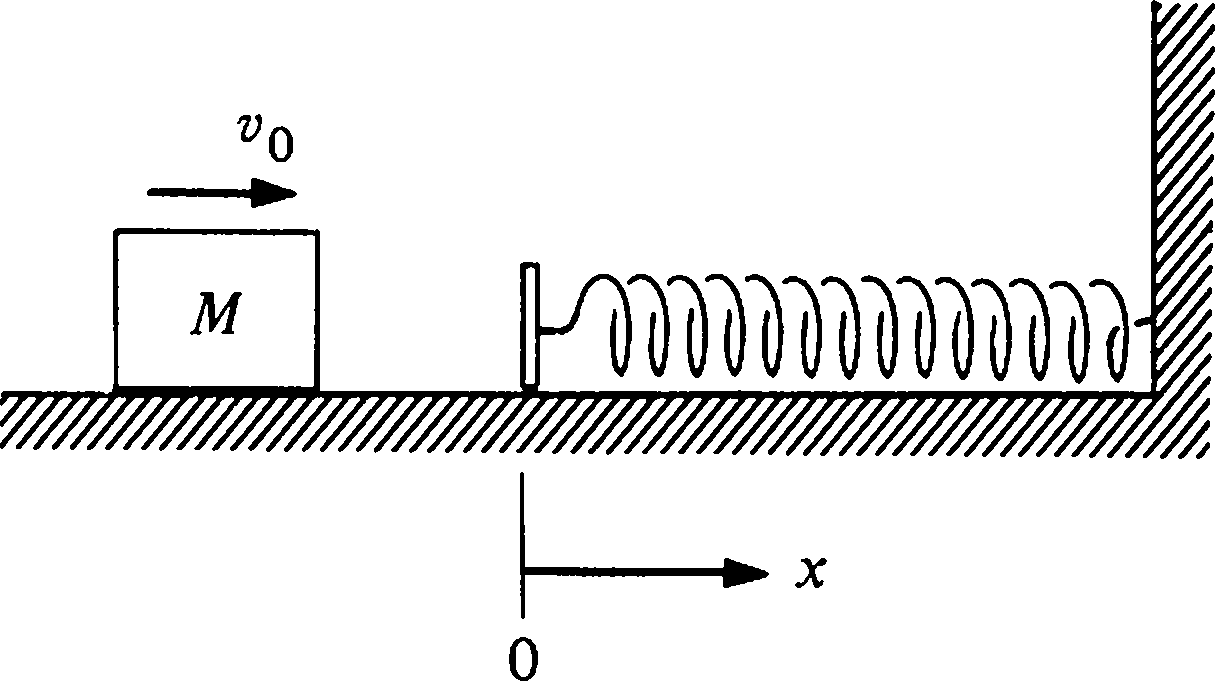
\includegraphics[width=0.4\textwidth]{ps06_1}\end{center}
\subsection*{Solution}
%\begin{align*}
%  m\dot v & = -bx m g - kx \\
%  \ddot x & = -\left(b g  + \frac{k}{m}\right)x \\
%  x(t) & = A\sin(\omega t) \\
%  \omega & = \sqrt{b g  + \frac{k}{m}} \\
%  x(t) & = A\sin\left(\sqrt{b g  + \frac{k}{m}}t\right) \\
%  \dot x(0) = v_0 & = A \\
%  x(t) & = v_0\sin\left(\sqrt{b g  + \frac{k}{m}}t\right) \\
%  0 & = \dot x(t_1) \\
%    & = v_0\sqrt{b g  + \frac{k}{m}}\cos\left(\sqrt{b g  + \frac{k}{m}}t_1\right) \\
%  2\pi n \pm \frac{\pi}{2} & = \sqrt{b g  + \frac{k}{m}}t_1 \\
%  \frac{\pi}{2} & = \sqrt{b g  + \frac{k}{m}}t_1 \\
%  t_1 & = \frac{\pi}{2}\cdot \sqrt{\frac{m}{m b g  + k}} \\
%  x(t_1) & = v_0
%\end{align*}
%FIX

\begin{align*}
  KE_0 & = \frac{1}{2}m v_0^2 \\
  \frac{\d KE_m}{\d x} & = -bx m g - kx \\
  \int_0^{KE_m(x)} \d{KE_m} & = \int_0^x {-bx m g - kx}\d x \\
  KE_m(x) - \frac{1}{2}m v_0^2 & = -\frac{1}{2}(b m g - k)x^2 \\
  KE_m(x) & = \frac{1}{2}m v_0^2 - \frac{1}{2}(b m g - k)x^2 \\
  \intertext{Since the object is at rest when $KE_m(x) = 0$,}
  KE_m(x_1) = 0 & = \frac{1}{2}m v_0^2 - \frac{1}{2}(b m g - k)x_1^2 \\
  \frac{1}{2}m v_0^2 & = \frac{1}{2}(b m g - k)x_1^2 \\
  x_1 & = \sqrt{\frac{m v_0^2}{b m g - k}} \\
  \\
  PE_0 & = 0 \\
  \frac{\d PE_s}{\d x} & = k x \\
  \int_0^{PE_s(x)} \d{PE_s} & = \int_0^x k x \d x \\
  PE_s(x) & = \frac{1}{2}k x^2 \\
  PE_s(x_1) & = \frac{1}{2}k x_1^2 \\
  PE_s(x_1) & = \frac{1}{2} k \left(\frac{m v_0^2}{b m g - k}\right) \\
   & = \frac{m v_0^2 k}{2(b m g - k)}
\end{align*}
\section*{Problem 2: K\&K 4.5}
\subsection*{Problem}
  A body of mass $m$ whirls around on a string which passes through a fixed ring located at the center of the circular motion. The string is held by a person who pulls the string downward with a constant velocity of magnitude $V$ so that the radial distance to the body decreases from an initial distance $r_0$ to a final distance $r_f$ from the center. The body has an initial angular velocity $\omega_0$. You may neglect the effect of gravity. Show that the work done in pulling the string equals the increase in kinetic energy of the body.
\subsection*{Solution}
  We want to show that $\displaystyle \int_{r_0}^{r_f}\vec F \cdot \vec d r = \Delta KE = \frac{1}{2}m\left((\omega r)^2 - (\omega_0 r_0)^2\right)$.
  \begin{align*}
  \vec r & = r \hat r \\
  \\
  \frac{\d \vec r}{\d t} & = \dot r\hat r + r\dot\theta\hat\theta \\
  \frac{\d \hat \theta}{\d t} & = -\dot\theta\hat r \\
  \\
  \frac{\d^2 \vec r}{\d t^2} & = \ddot r\hat r + \dot r\frac{\d \hat r}{\d t} + \dot r\dot\theta\hat\theta + r\ddot\theta\hat\theta + r\dot\theta\frac{\d \hat\theta}{\d t} \\
    & = \ddot r\hat r + \dot r\dot\theta\hat\theta + \dot r\dot\theta\hat\theta + r\ddot\theta\hat\theta - r\dot\theta^2\hat r \\
    & = (\ddot r - r\dot\theta^2)\hat r + (2\dot r\dot\theta + r\ddot\theta)\hat\theta \\
  \\
  \dot r & = -V \\
  \ddot r & = 0 \\
  \dot\theta & = \omega \\
  \frac{\d^2 \vec r}{\d t^2} & = -r\omega^2\hat r + (r\dot\omega - 2V\omega)\hat\theta \\
  \intertext{Since the force is radially inward, $r\dot\omega - 2V\omega = 0$.}
  \vec F & = -mr\omega^2\hat r \\
  \\
  r\dot\omega & = -2\dot r\omega \\
  -2\frac{\d r}{r} & = \frac{\d \omega}{\omega} \\
  -2\int_{r_0}^{r}\frac{\d r}{r} & = \int_{\omega_0}^{\omega(r)}\frac{\d \omega}{\omega} \\
  -2\ln\frac{r}{r_0} & = \ln\frac{\omega(r)}{\omega_0} \\
  \omega(r) & = \omega_0 \left(\frac{r_0}{r}\right)^2\\
  % \int_{t=0}^{t_f}\frac{2V}{r}\d t & = \int_{\omega_0}^{\omega_f}\frac{\d \omega}{\omega} \\
  % \frac{2V}{r}t_f & = \ln\frac{\omega_f}{\omega_0} \\
  % \omega(t) & = \omega_0 e^{\frac{2Vt}{r}} \\
  \\
  KE & = \frac{1}{2}mv^2 \\
    & = \frac{1}{2}m(\omega r)^2 \\
  \Delta KE & = \frac{1}{2}m\left((\omega_f r_f)^2 - (\omega_0 r_0)^2\right) \\
    & = \frac{1}{2}m\left((\omega_f r_f)^2 - (\omega_0 r_0)^2\right) \\
  \\
  W & = \int_{r_0}^{r_f} \vec F\cdot \vec {\d r} \\
    & = \int_{0}^{t_f} m(-r\omega^2\hat r)\cdot(\dot r\hat r + r\dot\theta\hat\theta)\d t \\
    & = m\int_{0}^{t_f} -r\omega^2\dot r \d t \\
  \intertext{Since $\d r = \dot r\d t$,}
    & = m\int_{r_0}^{r_f} -r\omega^2 \d r \\
  \intertext{Since $\omega(r) = \omega_0 \left(\frac{r_0}{r}\right)^2$,}
  W & = m\int_{r_0}^{r_f} -r\left(\omega_0 \left(\frac{r_0}{r}\right)^2\right)^2 \d r \\
    & = -m\omega_0^2r_0^4\int_{r_0}^{r_f} r^{-3} \d r \\
    & = \frac{1}{2}m\omega_0^2r_0^4\left(r_f^{-2} - r_0^{-2}\right) \\
    & = \frac{1}{2}m\left(r_0^2\left(\omega_0\frac{r_0}{r_f}\right)^{2} - (\omega_0 r_0)^2\right) \\
    & = \frac{1}{2}m\left(r_0^2\omega_0^2\left(\frac{r_0}{r_f}\right)^{2} - (\omega_0 r_0)^2\right) \\
    & = \frac{1}{2}m\left(r_0^2\omega_0\omega_f - (\omega_0 r_0)^2\right) \\
    & = \frac{1}{2}m\left(\frac{r_f^2r_0^2\omega_0}{r_f^2}\omega_f - (\omega_0 r_0)^2\right) \\
    & = \frac{1}{2}m\left((r_f\omega_f)^2 - (\omega_0 r_0)^2\right) \\
    & = \Delta KE
  \end{align*}%\\
  % \frac{\d \vec r}{\d t} & = \dot r\hat r + r\omega\hat\theta \\
  %  & = -V \hat r + r\omega\hat\theta \\
  % \\
  % \frac{\d \vec \theta}{\d t} & = -\dot\omega\hat\theta - \omega^2\hat r \\
  % \\
  % \\
  % \frac{\d^2 \vec r}{\d t^2} & = -V \frac{\d \hat r}{\d t} + r\dot\omega\hat\theta + \dot r\omega\hat\theta + r\omega\frac{\d \hat\theta}{\d t} \\ FIX
  %  & = -V \omega\hat\theta + r\dot\omega\hat\theta - V\omega\hat\theta - r\omega^2\hat r \\
  %  & = (r\dot\omega - 2V \omega)\hat\theta  - r\omega^2\hat r \\
  %  & = -V \omega\hat\theta + \dot\omega\hat\theta - \omega^2\hat r \\
  %  & = (\dot\omega - V \omega)\hat\theta - \omega^2\hat r \\
  %\end{align*}
\section*{Problem 3: K\&K 4.7}
\subsection*{Problem}
  A ring of mass $m_r$ hangs from a thread, and two identical beads of mass $m_b$ slide on it without friction. The beads are released simultaneously from the top of the ring and slide down opposite sides.
  \begin{center}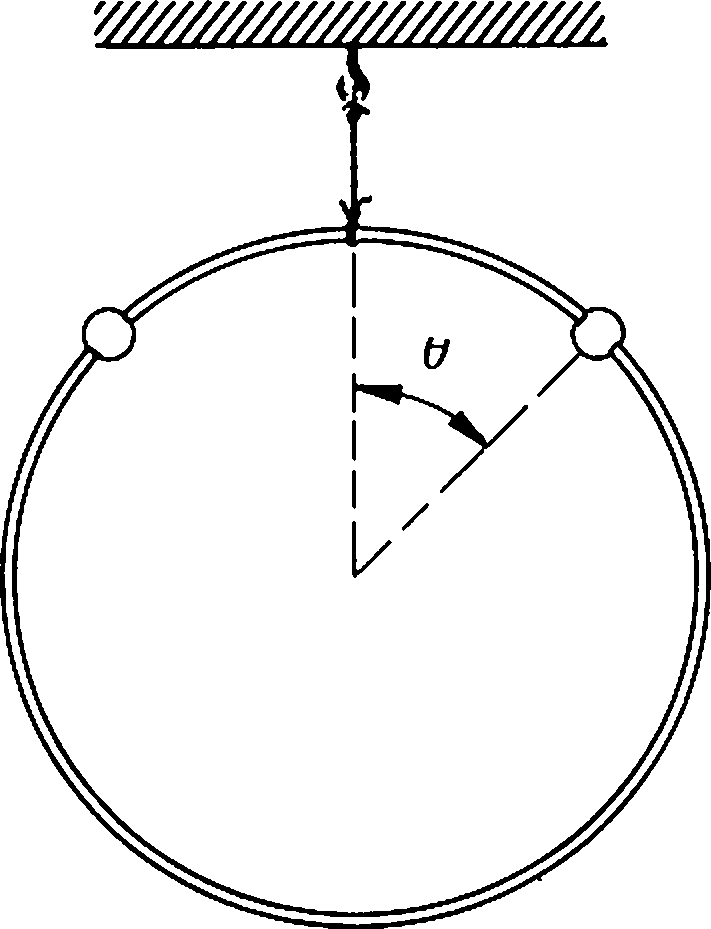
\includegraphics[width=0.2\textwidth]{ps06_2}\end{center}
  \begin{enumerate}[(a)]
  \item Draw free body force diagrams for the ring and the beads. What direction is the force of the bead on the ring pointing? Does it change has the bead moves. Can you still proceed with an analysis using Newton's Second Law if you are not sure which way this force points? Try to find a physical explanation for the direction of this force.
    \item Show that the ring will start to rise if $m_b > (3/2)m_r$, and find the angle $\theta$ with respect to the vertical direction that this occurs.
  \end{enumerate}
\subsection*{Solution}
\begin{enumerate}[a)]
 \item The direction should be in the radial direction, inward at the top, and outward at $\pi/2$ (because net force on the bead must be inward) and the bottom, and zero at $\cos\theta = \frac{2}{3}$ (see below) because the force should be perpendicular to the point of contact; the circle is locally linear.  It might be possible to do the analysis without knowing the angle. \par
 \begin{center}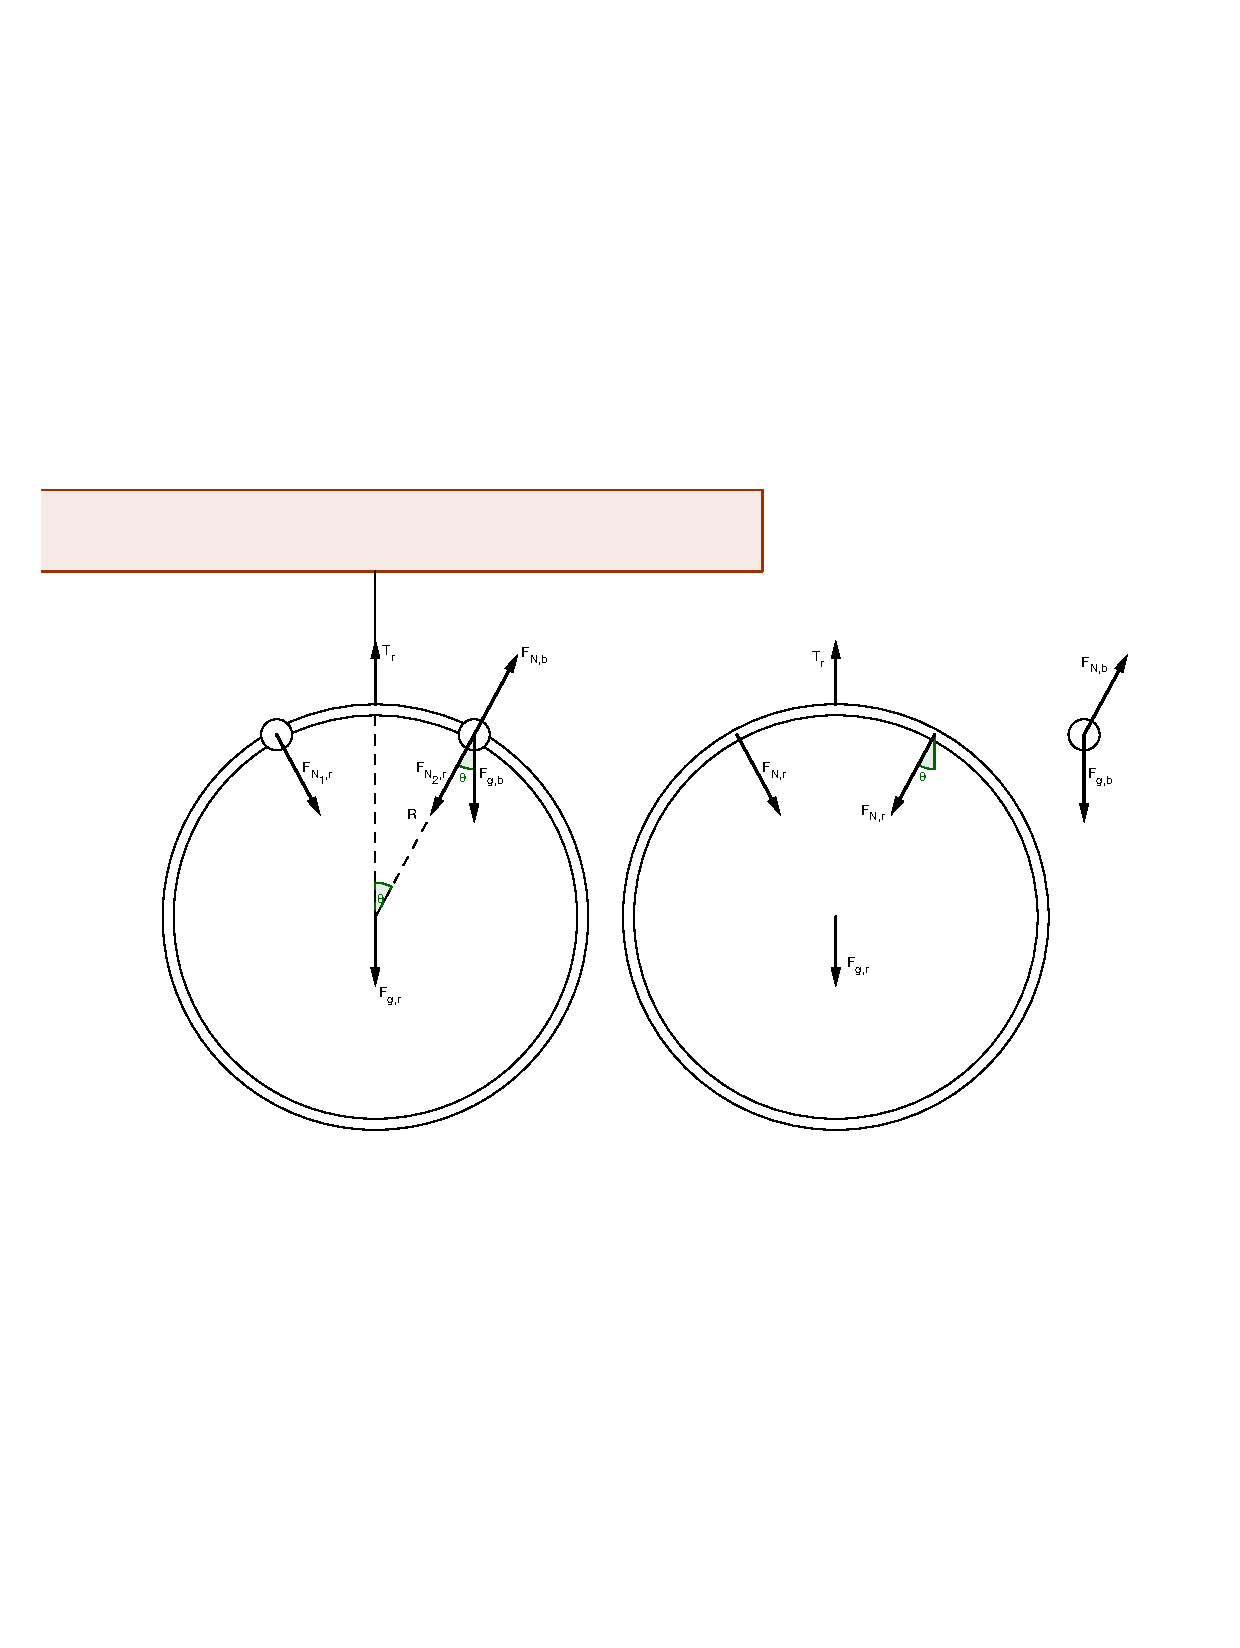
\includegraphics[width=0.75\textwidth]{2009-10-23_Diagram_7_1}\end{center}
 \item For the point at which the force is 0, $\frac{m_b v_b^2}{R} = m_b g\cos\theta$, so $\frac{v_b^2}{R} = g\cos\theta$.
   \begin{align*}
     0 & = \Delta PE + \Delta KE \\
       & = m_b g R(\cos\theta - 1) + \frac{1}{2}m_b v_b^2 \\
       & = 2 g R (\cos\theta - 1) + v_b^2 \\
     v_b^2 & = 2 g R(1 - \cos\theta) \\
     \intertext{Then, plugging into $\frac{v_b^2}{R} = g\cos\theta$,}
     \frac{2 g R(1 - \cos\theta)}{R} & = g\cos\theta \\
     2 (1 - \cos\theta) & = \cos\theta \\
     2 - 3\cos\theta & = 0 \\
     \cos\theta & = \frac{2}{3}
   \end{align*}
   For the ring,
   \begin{align*}
     m_r \vec a_r & = T\hat j - m_r g \hat j + 2 F_N\cos\theta \hat j \\
     \frac{\d \vec v_r}{\d t} & = \left(\frac{T}{m_r} + 2 \frac{F_N}{m_r}\cos\theta - g\right)\hat j
   \end{align*}
   At the instant the ring starts to rise, its acceleration is zero, and tension is zero.  Then, $2 \frac{F_N}{m_r}\cos\theta - g = 0$, so $$\cos\theta = \frac{m_r g}{2F_N}.$$
   For the bead,
   \begin{align*}
    m_b \vec a_b & = -m_b g\hat j -F_N\hat r \\
    \frac{\d \vec v_b}{\d t} & = -\left(g\cos\theta + \frac{F_N}{m_b}\right)\hat r + g\sin\theta\hat\theta  \\
    & = -g\hat j - \frac{F_N}{m_b}\cos\theta\hat j + \frac{F_N}{m_b}\sin\theta\hat i \\
    \\
    \frac{\d \vec r_b}{\d t} & = \dot R\hat r + R\dot\theta\hat\theta \\
     & = R\dot\theta\hat\theta \\
    \\
    \frac{\d^2 \vec r_b}{\d t^2} & = \dot R\dot\theta\hat \theta + R\ddot\theta\hat\theta + R\dot\theta \frac{\d\hat\theta}{\d t} \\
     & = \dot R\dot\theta\hat \theta + R\ddot\theta\hat\theta - R\dot\theta\dot\theta\hat r \\
     & = R\ddot\theta\hat\theta - R\dot\theta^2\hat r \\
    \\
    R\ddot\theta\hat\theta - R\dot\theta^2\hat r & = -\left(g\cos\theta + \frac{F_N}{m_b}\right)\hat r + g\sin\theta\hat\theta \\
    \\
    R\ddot\theta & = g\sin\theta \\
    -R\dot\theta^2 & = -\left(g\cos\theta + \frac{F_N}{m_b}\right) \\
    R\dot\theta^2 & = g\cos\theta + \frac{F_N}{m_b} \\
    \\
    \dot\theta^2 & = \frac{g}{R}\cos\theta + \frac{F_N}{m_b} \\
    \ddot\theta & = \frac{g}{R}\sin\theta
   \end{align*}

   Let the point at which potential energy is 0 be the final state, at which the ring begins to rise.  Then,
   \begin{align*}
    PE_{b, 0} & = 2 m_b g(R - R\cos\theta_f) \\
    KE_{b, 0} & = 0 \\
    PE_{b, f} & = 0 \\
    KE_{b, f} & = m_b v_f^2 \\
    \\
    2 m_b g(R - R\cos\theta_f) & = m_b v_f^2 \\
    2 R g(1 - \cos\theta_f) & = v_f^2 \\
    \cos\theta_f & = 1 - \frac{v_f^2}{2 R g}
   \end{align*}
   Then, we have the equations \begin{align*}
    \dot\theta_f^2 & = \frac{g}{R}\cos\theta_f + \frac{F_{N,f}}{R m_b} \\
    \ddot\theta_f & = \frac{g}{R}\sin\theta_f \\
    \cos\theta_f & = 1 - \frac{v_f^2}{2 R g} \\
    \cos\theta_f & = \frac{m_r g}{2F_{N,f}} \\
    v_f & = R \dot\theta_f
   \end{align*}
   Eliminating $\dot\theta_f$ and $\ddot\theta_f$,
   \begin{align*}
    \dot\theta_f^2 = \frac{v_f^2}{R^2} & = \frac{g}{R}\cos\theta_f + \frac{F_{N,f}}{R m_b} \\
    v_f^2 & = 2 R g(1 - \cos\theta_f) \\
    F_{N,f} & = \frac{m_r g}{2\cos\theta_f} \\
\intertext{Eliminating $v_f^2$,}
    v_f^2 = Rg\cos\theta_f + \frac{R F_{N,f}}{m_b} & = 2 R g(1 - \cos\theta_f) \\
    F_{N,f} & = \frac{m_r g}{2\cos\theta_f} \\
    \\
    m_b g\cos\theta_f + F_{N,f} & = 2 m_b g(1 - \cos\theta_f) \\
    F_{N,f} & = 2 m_b g - 2 m_b g \cos\theta_f - m_b g\cos\theta_f \\
    F_{N,f} & = m_b g(2 - 3\cos\theta_f) \\
     & = \frac{m_r g}{2\cos\theta_f} \\
    \frac{m_r}{2m_b} & = \cos\theta_f(2-3\cos\theta_f) \\
    \frac{m_r}{m_b} & = 2\cos\theta_f(2 - 3\cos\theta_f) \\
    0 & = -6\cos^2\theta_f + 4\cos\theta_f - \frac{m_r}{m_b} \\
    \cos\theta_f & = \frac{-4 \pm 2\sqrt{4-6\frac{m_r}{m_b}}}{-12} \\
     & = \frac{-2 \pm \sqrt{4-6\frac{m_r}{m_b}}}{-6} \\
     & = \frac{2 \pm \sqrt{4-6\frac{m_r}{m_b}}}{6} \\
\intertext{Since the rising must happen between when the normal force is zero and when it's in the $\hat i$ direction, $\frac{2}{3} \geq \cos\theta_f \geq 0$.}
    \frac{m_r}{m_b} & = 2\cos\theta_f(2 - 3\cos\theta_f) \\
\intertext{Taking the derivative, and setting it equal to zero,}
    0 & = -4\sin\theta_f + 12\cos\theta_f\sin\theta_f \\
      & = -1\sin\theta_f + 3\cos\theta_f\sin\theta_f \\
\intertext{Since $\sin\theta_f \neq 0$ ($\theta_f\neq 0, \pi$),}
    0 & = 3\cos\theta_f - 1 \\
    \cos\theta_f & = \frac{1}{3} \\
    \\
    \frac{m_r}{m_b} & = 2\cdot\frac{1}{3}(2 - 3\cdot\frac{1}{3}) \\
     & = \frac{2}{3} \\
   \end{align*}
   Then $m_b > \frac{3}{2}m_r$.
% Because, while the ring is not moving, tension does no work, energy is conserved in the earth and ring system.  Then,
%   \begin{align*}
%   \vec r_{\text{CM}} & = \frac{2m_b R\cos\theta}{2m_b + m_r}\hat j \\
%   \\
%%   (2m_b + m_r)g & = \frac{\d \frac{2m_b R\cos\theta}{2m_b + m_r}
%   \vec v_{\text{CM}} & = -\frac{2m_b R}{2m_b + m_r}\sin\theta\dot\theta\hat j \\
%   \\
%   0 & = \Delta KE + \Delta PE \\
%     & = \frac{1}{2}(2m_b + m_r)\left(\frac{2m_b R}{2m_b + m_r}\right)^2\left(\left(\sin\theta_f\theta'_f\right)^2 - \left(\sin 0\theta'_0\right)^2\right) + (2m_b + m_r)Rg(\cos\theta_f - \cos 0) \\
%     & = \frac{2m_b^2 R^2}{2m_b + m_r}\sin^2\theta_f(\theta'_f)^2 + (2m_b + m_r)Rg(\cos\theta_f - 1) \\
%     & = 2R\left(\frac{m_b }{2m_b + m_r}\right)^2(1-\cos^2\theta_f)(\theta'_f)^2 + g(\cos\theta_f - 1) \\
%   \end{align*}\begin{align*}
%   1 - \cos\theta_f & = \frac{2R}{g}\left(\frac{m_b }{2m_b + m_r}\right)^2(1-\cos^2\theta_f)(\theta'_f)^2 \\
%   \frac{1 - \cos\theta}{1-\cos^2\theta} & = \frac{2R}{g}\left(\frac{m_b }{2m_b + m_r}\right)^2\left(\frac{\d \theta}{\d t}\right)^2 \\
%   \frac{1}{1+\cos\theta} & = \frac{2R}{g}\left(\frac{m_b}{2m_b + m_r}\right)^2\left(\frac{\d \theta}{\d t}\right)^2 \\
%   \frac{\d \theta}{\d t} & = \pm\frac{2m_b + m_r}{2m_b}\sqrt{\frac{2g}{R(1+\cos\theta)}} \\
%   \\
%   \vec v_{CM} & = -\frac{2m_b R}{2m_b + m_r}\sin\theta\theta' \hat j \\
%               & = -\frac{2m_b R}{2m_b + m_r}\sin\theta\left(\pm\frac{2m_b + m_r}{2m_b}\sqrt{\frac{2g}{R(1+\cos\theta)}}\right) \hat j \\
%               & = \mp\frac{2m_b R}{2m_b + m_r}\cdot\frac{2m_b + m_r}{2m_b}\sin\theta\sqrt{\frac{2g}{R(1+\cos\theta)}} \hat j \\
%               & = \mp R\sin\theta\sqrt{\frac{2g}{R(1+\cos\theta)}} \hat j \\
%               & = \mp \sin\theta\sqrt{\frac{2gR}{1+\cos\theta}} \hat j \\
%               & = \mp \sqrt{\frac{2gR(1 - \cos^2\theta)}{1+\cos\theta}} \hat j \\
%               & = \mp \sqrt{2gR(1 - \cos\theta)} \hat j \\
%               & = \mp R\sqrt{\frac{2g(1-\cos^2\theta)}{R(1+\cos\theta)}} \hat j \\
%               & = \mp \sqrt{2gR(1-\cos\theta)} \hat j \\
%   \vec v_{CM} & = -\sqrt{2gR(1-\cos\theta)} \hat j \\
%               & = -2\sqrt{gR\frac{1-\cos\theta}{2}} \hat j \\
%               & = -2\sqrt{gR\sin^2\frac{\theta}{2}} \hat j \\
%               & = -2\sqrt{gR}\sin\frac{\theta}{2} \hat j \\
%               & = -2\sqrt{gR}\sin\frac{\theta}{2} \hat j
%   \end{align*} Since the normal force on the beads is perpendicular to the instantaneous direction of motion, the only nonconservative force doing work on the beads is gravity.  Then,
%   \begin{align*}
%    \int_R^{R\cos\theta}\vec F \cdot \vec d r & = \Delta KE \\
%     & = \frac{1}{2}\cdot 2m_b v_b^2 \\
%     & = m_b v_b^2 \\
%    \int_R^{R\cos\theta}\vec F \cdot \vec d r & = \int_0^{\theta}-2m_b g R\cos\theta d \theta \\
%     & = -2m_b g R(\cos\theta - 1) \\
%     & = 2m_b g R(1 - \cos\theta) \\
%     & = m_b v_b^2 \\
%    v_b^2 & = 2 g R(1 - \cos\theta) \\
%    v_b & = \sqrt{2 g R(1 - \cos\theta)} \\
%   \end{align*}
%   While the ring is not in motion, the kinetic energy of the the system is the sum of the kinetic energies of the beads.  Then,
%   \begin{align*}
%    \frac{1}{2}(2m_b + m_r)\left(-2\sqrt{gR}\sin\frac{\theta}{2}\right)^2 & = \frac{1}{2}\cdot 2m_b\sqrt{2 g R(1 - \cos\theta)}^2 \\
%    (2m_b + m_r)4gR\sin^2\frac{\theta}{2} & = 2m_b(2 g R(1 - \cos\theta)) \\
%    (2m_b + m_r)\sin^2\frac{\theta}{2} & = m_b(1 - \cos\theta) \\
%    (2m_b + m_r)\frac{1}{2}(1-\cos\theta) & = m_b(1 - \cos\theta) \\
%    (2m_b + m_r) & = 2m_b \\
%    m_r & = 0
%   \end{align*}
\end{enumerate}
\section*{Problem 4: K\&K 4.9}
\subsection*{Problem}
  Consider the exothermic reaction (final kinetic energy is greater than the initial kinetic energy).
  $$\text{H} + \text{H} \to \text{H}_2 + 5\text{ eV}$$
  Two hydrogen atoms collide and produce a diatomic hydrogen molecule. However, when hydrogen atoms collide in free space they simply bounce apart. The reason is that it is impossible to satisfy the laws of conservation of energy and momentum in a simple two body collision which releases energy.
  \begin{enumerate}[(a)]
  \item Can you prove this? Try to analyze this collision in a reference frame moving with the velocity of the center of mass of the system.
    \item Can this two body reaction take place if the temperature is dramatically lowered to near zero degrees Kelvin? Try to give an physical explanation for your answer.
  \end{enumerate}
\subsection*{Solution}
  \begin{enumerate}[(a)]
  \item If the center of mass is not moving, then the $v_A = -v_B$.  Then $m v_A - m v_A = 2 m v'$, so $v = 0$.  Then the kinetic energy is lower, which contradicts the assumption that the reaction is exothermic.
    \item $m(\vec v_A + \vec v_B) = 2 m \vec v_f$, and $mv_f^2 = \frac{1}{2}m(v_A^2 + v_B^2) + 5\text{ eV}$.  Then $v_f^2 = \frac{v_A^2 + v_B^2 + 2\vec v_A \cdot \vec v_B}{4} = \frac{v_A^2 + v_B^2}{2} + 5\text{ eV}$.  Then $v_A^2 + v_B^2 + 2\vec v_A \cdot \vec v_B = 2v_A^2 + 2v_B^2 + 20\text{ eV}$.  Then $-20\text{ eV} = (\vec v_A - \vec v_B)\cdot(\vec v_A - \vec v_B)$, which is impossible, regardless of how small the velocities are.
  \end{enumerate}
\section*{Problem 5: K\&K 4.10}
\subsection*{Problem}
  A block of mass $m_b$ on a horizontal table is connected to one end of a spring with spring constant $k$. The other end of the spring is attached to a wall. The block is set in motion so that it oscillates about its equilibrium point with amplitude $A_0$.
  \begin{enumerate}[(a)]
  \item What is the period of the motion?
    \interitemtext{A lump of sticky putty of mass $m_p$ is dropped onto the block. The putty sticks without bouncing. The putty hits the block at the instant when the velocity of the block is zero.}
    \item Find the new period, the new amplitude, and the change in mechanical energy of the system.
    \interitemtext{The putty is removed and the block is set in motion. This time the putty is dropped and hits the block at the instant the block has its maximum velocity.}
    \item Find the new period, the new amplitude, and the change in mechanical energy of the system.
  \end{enumerate}
\subsection*{Solution}
  \begin{enumerate}[a)]
    \item $\frac{\d^2 x}{\d t^2} = -\frac{k}{m_b}x$, $x = A_0\sin(\omega t)$, so $\omega = \sqrt{\frac{k}{m_b}}$.  Then the period is $2\pi \sqrt{\frac{m_b}{k}}$
    \item There is no change in the energy at the moment of impact, so there's no change in mechanical energy, so the new amplitude is still $A_0$, and the new period is $2\pi\sqrt{\frac{m_b + m_p}{k}}$.
    \item The new period is $2\pi\sqrt{\frac{m_b + m_p}{k}}$.  The maximum velocity is $\sqrt{2\frac{KE}{m_b}} = \sqrt{2\frac{PE_{\text{max}}}{m_b}} = \sqrt{\frac{k A_0^2}{4m_b}} = \frac{A_0}{2} \sqrt{\frac{k}{m_b}}$.  Then the new velocity is $\frac{m_b\frac{A_0}{2}\sqrt{\frac{k}{m_b}}}{m_b + m_p} = \frac{\frac{A_0}{2}\sqrt{k m_b}}{m_b + m_p}$.  Then the new kinetic energy is $\frac{1}{2}(m_b + m_p)\frac{A_0^2}{4}\frac{k m_b}{(m_b + m_p)^2} = \frac{A_0^2}{4}\frac{k m_b}{m_b + m_p}$ (as compared to $\frac{1}{2}k \frac{A_0^2}{4}$).  Then the new amplitude is $A_0\sqrt{\frac{m_b}{m_b + m_p}}$.
  \end{enumerate}
\section*{Problem 6: K\&K 4.12}
\subsection*{Problem}
  During the Second World War the Russians, lacking sufficient parachutes for airborne operations, occasionally dropped soldiers inside bales of hay onto snow. The human body can survive an average pressure of 30 lbs / in$^2$. Suppose that the lead plane drops a dummy bale equal in weight to a loaded one from an altitude of 150 ft, and that the pilot observes that it sinks about 2 ft into the snow. If the weight of an average soldier is 144 lbs and his effective area is 5 ft$^2$, is it safe to drop the men?
\subsection*{Solution}
  \begin{align*}
    \int_{2\text{ ft}}^{0\text{ ft}} \vec F \cdot \vec d r & = m g h \\
    & = (144\text{ lbs})(152\text{ ft}) \\
    \int_{2\text{ ft}}^{0\text{ ft}} F d h & = 21888\text{ ft lbs}
  \end{align*}
  In the best case scenario, when force is constant for the duration of motion in the snow, $F = 10944\text{ lbs}$.  5 ft$^2$ is 720 in$^2$, so $P = 15.2\text{ lbs / in}^2$.  FIX?
\section*{Problem 7: K\&K 4.13}
\subsection*{Problem}
  A commonly used potential energy function to describe the interaction between two atoms is the Lennard-Jones 6,12 potential
  $$U(r) = \varepsilon\left[(r_0 / r)^{12} - 2(r_0 / r)^6\right].$$
  \begin{enumerate}[(a)]
  \item Show that the radius at the potential minimum is $r_0$, and that the depth of the potential well is $\varepsilon$.
    \item Find the angular frequency of small oscillations about the stable equilibrium position for two identical atoms of mass $m$ bound to each other by the Lennard-Jones interaction.
  \end{enumerate}
\subsection*{Solution}
\begin{enumerate}[a)]
  \item The minimum is at $U'(r) = 0$, so $\epsilon\left[-12(r / r_0)^{-13} + 12(r / r_0)^{-7}\right] = 0$, so $(r / r_0)^{13} = (r / r_0)^{7}$, or $(r / r_0)^6 = 1$.  Then $r = r_0$.  Then $U(r_0) = \epsilon(1^12 - 2\cdot 1^6) = -\epsilon$.
  \item Approximate the potential function as $U(r) = U(r_0) + \left.\frac{\d U}{\d r}\right|_{r=r_0}(r-r_0) + \left.\frac{\d^2 U}{\d r^2}\right|_{r=r_0}(r-r_0)^2$.  Since $\left.\frac{\d U}{\d r}\right|_{r=r_0}(r-r_0) = 0$, $U(r) = -\epsilon + \left.\frac{\d^2 U}{\d r^2}\right|_{r=r_0}(r-r_0)^2$.  $\left.\frac{\d^2 U}{\d r^2}\right|_{r=r_0} = \epsilon\left[12\cdot 13 (r_0 / r_0)^{-14} -12\cdot 7(r_0/r_0)^{-8}\right] = \epsilon(12\cdot 6) = 72\epsilon$.  Then $U(r) = -\epsilon + 72\epsilon(r - r_0)^2$. \par
  Then $E = \frac{1}{2}\mu\left(\frac{\d r}{\d t}\right)^2 + U(r_0) + \frac{1}{2}k(r-r_0)^2$.  Then $\frac{\d E}{\d t} = 0 = \mu\left(\frac{\d r}{\d t}\right)\left(\frac{\d^2 r}{\d t^2}\right) + k(r - r_0)\frac{\d r}{\d t}$.  Then $\frac{\d r}{\d t}\left(\mu \left(\frac{\d^2 r}{\d t^2}\right) + k(r - r_0)\right) = 0$, so $\frac{\d^2 r}{\d t^2} = -\frac{k}{\mu}(r - r_0)$, the frequency of oscillation is $\sqrt{\frac{\frac{k}{\mu}}} = \sqrt{\frac{72\epsilon}{m / 2}} = \sqrt{\frac{144\epsilon}{m}}$.
  %
  %$KE_{r_{\text{min}}} + PE_{r_{\text{min}}} = KE_{r_0} + PE_{r_0} = PE_{r_{\text{max}}} + KE_{r_{\text{max}}}$.  $KE_{r_{\text{max}}} = KE_{r_{\text{min}}} = 0$.  Then $PE_{r_{\text{min}}}  = KE_{r_0} - \epsilon = PE_{r_{\text{max}}}$.  Then $\epsilon\left[(r_0 / r_{\text{min}})^{12} - 2(r_0 / r_{\text{min}})^6\right] = 2\cdot \frac{1}{2} m v_{r_0}^2 - \epsilon = \epsilon\left[(r_0 / r_{\text{max}})^{12} - 2(r_0 / r_{\text{max}})^6\right]$.  Then $(r_0 / r_{\text{min}})^{12} - 2(r_0 / r_{\text{min}})^6 = \frac{m}{\epsilon}v_{r_0}^2 - 1 = (r_0 / r_{\text{max}})^{12} - 2(r_0 / r_{\text{max}})^6$.  FIX
\end{enumerate}
\end{document}
